\section{Une supervision générique orientée données}\label{sec:intro:objectif}
Il existe de nombreux produits commerciaux ou académiques de supervision pour effectuer des taches de surveillances notamment dans le cadre de la gestions de serveurs (d'un point de vue réseau~\cite{gestionequipreseau} ou applicatif~\cite{supervisionapache}), la gestion de processus opérationnels d'entreprises~\cite{google:businessprocesssupervision} et l'administration d'un parc de dispositifs~\cite{snmp:thesemehdi}. Cependant, les approches actuelles ont différents problèmes majeurs :
\begin{itemize}
    \item \textbf{Restriction à une perspective} : comme vu précédemment, la supervision doit s'adapter aux différents systèmes et aux différents angles de vues possibles. Plusieurs solutions ne se focalisent que sur un cœur de métier en particulier, rendant l'ensemble très ad-hoc et peu réutilisable.
    \item \textbf{Vision unilatérale} : l'observation ne se fait que sur une seule entité du système (un ensemble de données d'un équipement). Le système n'est pas considéré comme un tout rendant la compréhension des interactions entre les entités du système difficile.
    \item \textbf{Focalisation forte sur le processus de collecte} : en l'état, beaucoup de travaux ont été effectués pour permettre aux solutions d'administrations d'accéder aux équipements. Ceci, certes, permet l'accès aux données mais ouvre la porte à une gestion difficile de la masse ainsi obtenue.
    \item \textbf{Gestion de l'évolution des données limitée} : deux approches principales sont utilisées en l'état. Soit le traitement des données se fait \textit{à chaud} par l'observation d'une fenêtre de temps limitée permettant ainsi de favoriser les solutions proactive pour notamment faire des systèmes d'alerte. Soit les données sont archivées pour en faire le traitement plus complexe par la suite en vu d'une analyse plus poussée. Il est très rare de voir un système d'observation capable de gérer ces deux approches de façon unifiée. 
\end{itemize}

\begin{figure}
\centering
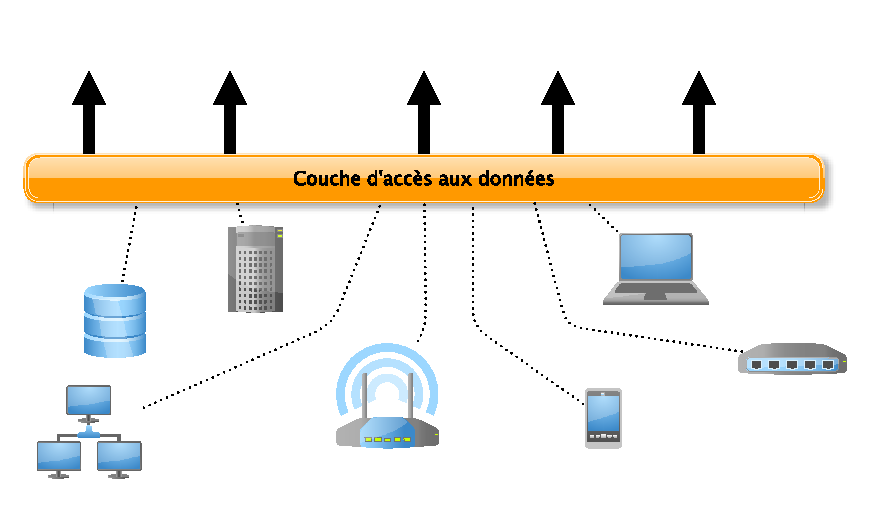
\includegraphics[width=0.7\textwidth]{intro-objectif}
\caption{Couche d'abstraction du système pour donner accès aux données}\label{fig:intro:objectif:abstraction}
\end{figure}

L'objectif final de cette thèse est d'obtenir une supervision générique permettant de répondre à la grande hétérogénéité présentée en section~\ref{sec:intro:problematique}. Contrairement aux approches actuelles, il est ici considéré comme acquis le fait de pouvoir dialoguer d'une manière ou d'une autre avec les dispositifs de manière à récolter les données. La figure~\ref{fig:intro:objectif:abstraction} représente la couche d'abstraction du système, permettant un accès unifié aux données. Le système est donc considéré comme un ensemble de sources de données hétérogènes qu'il nous faut maîtriser. Chacune de ces sources exposant un fragment de l'ensemble des données du système. Ce positionnement est principalement motivé par la grande quantité de travaux effectués sur le sujet et du fait que les dispositifs, même grand publique, permettent de plus en plus des accès standards à leurs canaux de données (voir section~\ref{sec:rw:supervision:administration}). Ainsi, cette thèse n'aborde pas les problématiques (complexes) d'hétérogénéité de protocoles de communications pour permettre l'accès aux données.

Cette gestion de données sera donc l'interface entre le système à observer et les différents utilisateurs (humains ou machines). Ce système permettra ainsi de créer des processus de collecte et de traitement de manière la plus flexible possible. Voici les caractéristiques que la solution se doit de respecter pour répondre à notre problématique :
\begin{itemize}
    \item \textbf{Applicable sur tout type de système} : l'approche ne doit pas considérer comme acquis un type de système ou un cœur de métier en particulier. En effet, comme présenté précédemment, un des problèmes majeurs rencontrés dans les solutions existantes est la restriction à une perspective.
    \item \textbf{Langage unifié} : il est nécessaire que les processus de traitement des données doivent être écrits dans un seul et même langage. Ce langage doit être capable de traiter l'hétérogénéité sur les données, y compris au niveau temporelle. En effet, le système de supervision mêlera données statiques et dynamiques sur lesquelles serons exécutés des traitements continus ou instantanés, le langage doit être capable d'exprimer proprement ces processus.
    \item \textbf{Extensible} : si l'utilisateur souhaite pouvoir implémenter une nouvelle fonctionnalité afin de mieux adapter la solution à son cas d'usage, il doit avoir la possibilité de le faire. Ceci peut avoir un impact pour pouvoir par exemple effectuer un traitement spécifique à un métier, ou encore pour améliorer les performances dans un cadre particulier. Ainsi, il sera plus facile d'intégrer le système de supervision avec son cadre d'utilisation.
    \item \textbf{Performant} : l'exécution des processus doit pouvoir se faire de manière suffisamment efficace. L'aspect performance est à considéré car que ce soit pour le passage à l'échelle ou à l'inverse le déploiement sur dispositifs embarqué, la quantité de ressources nécessaire pour exécuter un processus doit être contrôlé.
\end{itemize}
